%!TEX root = ../document.tex

During our interviews, we briefly observed Christof Dorner from Readmill during his work. He showed us how he develops a feature: He picks a task from the bug and feature tracker \emph{Trello}, creates a \emph{git} branch locally, fixes the problem and writes tests for it. Eventually he opens a Pull Request on Github for the finished code to be reviewed and deployed. Here we gained the insight, that a frictionless and uninterrupted flow is highly valuable. This can be achieved by customizing and constantly improving the used tools. Christof mentioned how he improved his flow over time, e.g. making tests run instantly on each change or working with a decentralized source code management tool.

We also had the chance to observe the two current EPIC chair's Bachelor project teams. Both work with real customer data as well as existing legacy code. During observation we noticed that one issue they face is a disconnect between understanding the code in the editor and the data in the database. This leads to switching back and forth between the code editor and the \emph{HANA Database Studio} as well as guessing values for variables in the queries.

Additionally to the interviews and observations, we took into account our own experience of developing applications with databases as well as incoorperated experiences from the seminar \emph{Enterprise Application Programming Model Research 2012} at the HPI EPIC chair~\footnote{\url{https://github.com/lauritzthamsen/infrarecord/}}.

\begin{figure}
    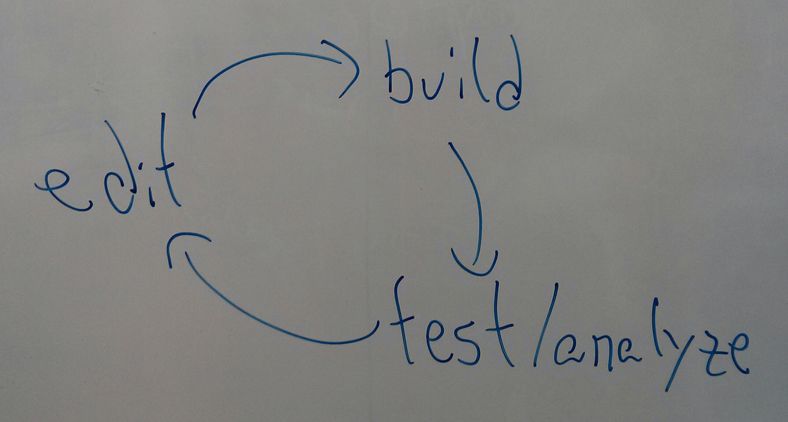
\includegraphics[width=\linewidth]{images/EditBuildTest.jpg}
    \caption{The code development cycle drawn on a whiteboard during the project week}
    \label{fig:cycle}
\end{figure}

While investigating common workflows of software developers, we realized that they often follow the cycle depicted in Figure~\ref{fig:cycle}. Before entering that cycle, the software developer chooses the scope of a certain feature and does all the necessary work to have an actionable coding task at hand. The cycle is only started when the actual code generation begins. Depending on the programming language, the developer has to build the code or otherwise bring it into a testable state. In a next step he tests the changes made, e.g. through unit tests or by executing and manually testing the application. This cycle repeats, until the developer is satisfied with the results.

Once this cycle became apparent to us, we investigated the components it operates on. Especially from the experiences of the bachelor project teams let us realize, that, while in the editing step, the developer has no access to the data context in which the code will eventually be executed during the test \& analyze step. There is a disconnect between the editor and the application runtime. In the editing step the developer writes down his or her thoughts as code but only later on will it be interpreted by the machine. For the same reason the cycle exists in the first place. Because developers have to continuously test the assumptions they made about the behavior of their program. We learned, that every execution of the cycle is an interruption to the developer. Instead, we consider a cycle, which is so fluent that moving from one step to another becomes barely noticeable, the far better solution. One important requirement for this would that already during coding, the developer has access to the context the program will finally be executed in. When working with an external data source, the actual data can act as this valuable context.

Once aware of these conclusions, we developed our third insight, which also guided us through the rest of our project:

\begin{quote}
\emph{Code needs data context}
\end{quote}